\documentclass[]{article}
\usepackage{lmodern}
\usepackage{amssymb,amsmath}
\usepackage{ifxetex,ifluatex}
\usepackage{fixltx2e} % provides \textsubscript
\ifnum 0\ifxetex 1\fi\ifluatex 1\fi=0 % if pdftex
  \usepackage[T1]{fontenc}
  \usepackage[utf8]{inputenc}
\else % if luatex or xelatex
  \ifxetex
    \usepackage{mathspec}
  \else
    \usepackage{fontspec}
  \fi
  \defaultfontfeatures{Ligatures=TeX,Scale=MatchLowercase}
\fi
% use upquote if available, for straight quotes in verbatim environments
\IfFileExists{upquote.sty}{\usepackage{upquote}}{}
% use microtype if available
\IfFileExists{microtype.sty}{%
\usepackage{microtype}
\UseMicrotypeSet[protrusion]{basicmath} % disable protrusion for tt fonts
}{}
\usepackage[margin=1in]{geometry}
\usepackage{hyperref}
\hypersetup{unicode=true,
            pdftitle={Chapter Three},
            pdfauthor={Ryan Honea},
            pdfborder={0 0 0},
            breaklinks=true}
\urlstyle{same}  % don't use monospace font for urls
\usepackage{color}
\usepackage{fancyvrb}
\newcommand{\VerbBar}{|}
\newcommand{\VERB}{\Verb[commandchars=\\\{\}]}
\DefineVerbatimEnvironment{Highlighting}{Verbatim}{commandchars=\\\{\}}
% Add ',fontsize=\small' for more characters per line
\usepackage{framed}
\definecolor{shadecolor}{RGB}{248,248,248}
\newenvironment{Shaded}{\begin{snugshade}}{\end{snugshade}}
\newcommand{\KeywordTok}[1]{\textcolor[rgb]{0.13,0.29,0.53}{\textbf{{#1}}}}
\newcommand{\DataTypeTok}[1]{\textcolor[rgb]{0.13,0.29,0.53}{{#1}}}
\newcommand{\DecValTok}[1]{\textcolor[rgb]{0.00,0.00,0.81}{{#1}}}
\newcommand{\BaseNTok}[1]{\textcolor[rgb]{0.00,0.00,0.81}{{#1}}}
\newcommand{\FloatTok}[1]{\textcolor[rgb]{0.00,0.00,0.81}{{#1}}}
\newcommand{\ConstantTok}[1]{\textcolor[rgb]{0.00,0.00,0.00}{{#1}}}
\newcommand{\CharTok}[1]{\textcolor[rgb]{0.31,0.60,0.02}{{#1}}}
\newcommand{\SpecialCharTok}[1]{\textcolor[rgb]{0.00,0.00,0.00}{{#1}}}
\newcommand{\StringTok}[1]{\textcolor[rgb]{0.31,0.60,0.02}{{#1}}}
\newcommand{\VerbatimStringTok}[1]{\textcolor[rgb]{0.31,0.60,0.02}{{#1}}}
\newcommand{\SpecialStringTok}[1]{\textcolor[rgb]{0.31,0.60,0.02}{{#1}}}
\newcommand{\ImportTok}[1]{{#1}}
\newcommand{\CommentTok}[1]{\textcolor[rgb]{0.56,0.35,0.01}{\textit{{#1}}}}
\newcommand{\DocumentationTok}[1]{\textcolor[rgb]{0.56,0.35,0.01}{\textbf{\textit{{#1}}}}}
\newcommand{\AnnotationTok}[1]{\textcolor[rgb]{0.56,0.35,0.01}{\textbf{\textit{{#1}}}}}
\newcommand{\CommentVarTok}[1]{\textcolor[rgb]{0.56,0.35,0.01}{\textbf{\textit{{#1}}}}}
\newcommand{\OtherTok}[1]{\textcolor[rgb]{0.56,0.35,0.01}{{#1}}}
\newcommand{\FunctionTok}[1]{\textcolor[rgb]{0.00,0.00,0.00}{{#1}}}
\newcommand{\VariableTok}[1]{\textcolor[rgb]{0.00,0.00,0.00}{{#1}}}
\newcommand{\ControlFlowTok}[1]{\textcolor[rgb]{0.13,0.29,0.53}{\textbf{{#1}}}}
\newcommand{\OperatorTok}[1]{\textcolor[rgb]{0.81,0.36,0.00}{\textbf{{#1}}}}
\newcommand{\BuiltInTok}[1]{{#1}}
\newcommand{\ExtensionTok}[1]{{#1}}
\newcommand{\PreprocessorTok}[1]{\textcolor[rgb]{0.56,0.35,0.01}{\textit{{#1}}}}
\newcommand{\AttributeTok}[1]{\textcolor[rgb]{0.77,0.63,0.00}{{#1}}}
\newcommand{\RegionMarkerTok}[1]{{#1}}
\newcommand{\InformationTok}[1]{\textcolor[rgb]{0.56,0.35,0.01}{\textbf{\textit{{#1}}}}}
\newcommand{\WarningTok}[1]{\textcolor[rgb]{0.56,0.35,0.01}{\textbf{\textit{{#1}}}}}
\newcommand{\AlertTok}[1]{\textcolor[rgb]{0.94,0.16,0.16}{{#1}}}
\newcommand{\ErrorTok}[1]{\textcolor[rgb]{0.64,0.00,0.00}{\textbf{{#1}}}}
\newcommand{\NormalTok}[1]{{#1}}
\usepackage{longtable,booktabs}
\usepackage{graphicx,grffile}
\makeatletter
\def\maxwidth{\ifdim\Gin@nat@width>\linewidth\linewidth\else\Gin@nat@width\fi}
\def\maxheight{\ifdim\Gin@nat@height>\textheight\textheight\else\Gin@nat@height\fi}
\makeatother
% Scale images if necessary, so that they will not overflow the page
% margins by default, and it is still possible to overwrite the defaults
% using explicit options in \includegraphics[width, height, ...]{}
\setkeys{Gin}{width=\maxwidth,height=\maxheight,keepaspectratio}
\IfFileExists{parskip.sty}{%
\usepackage{parskip}
}{% else
\setlength{\parindent}{0pt}
\setlength{\parskip}{6pt plus 2pt minus 1pt}
}
\setlength{\emergencystretch}{3em}  % prevent overfull lines
\providecommand{\tightlist}{%
  \setlength{\itemsep}{0pt}\setlength{\parskip}{0pt}}
\setcounter{secnumdepth}{0}
% Redefines (sub)paragraphs to behave more like sections
\ifx\paragraph\undefined\else
\let\oldparagraph\paragraph
\renewcommand{\paragraph}[1]{\oldparagraph{#1}\mbox{}}
\fi
\ifx\subparagraph\undefined\else
\let\oldsubparagraph\subparagraph
\renewcommand{\subparagraph}[1]{\oldsubparagraph{#1}\mbox{}}
\fi

%%% Use protect on footnotes to avoid problems with footnotes in titles
\let\rmarkdownfootnote\footnote%
\def\footnote{\protect\rmarkdownfootnote}

%%% Change title format to be more compact
\usepackage{titling}

% Create subtitle command for use in maketitle
\newcommand{\subtitle}[1]{
  \posttitle{
    \begin{center}\large#1\end{center}
    }
}

\setlength{\droptitle}{-2em}
  \title{Chapter Three}
  \pretitle{\vspace{\droptitle}\centering\huge}
  \posttitle{\par}
  \author{Ryan Honea}
  \preauthor{\centering\large\emph}
  \postauthor{\par}
  \predate{\centering\large\emph}
  \postdate{\par}
  \date{9/8/2017}

\usepackage{bbm}

\begin{document}
\maketitle

\subsection{Exercise One}\label{exercise-one}

\paragraph{Question}\label{question}

The following relationships can be described by generalized linear
models. For each one, identify the response variable and the explanatory
variables, select a probability distribution for the response
(justifying your choice) and write down the linear component.

\paragraph{Solutions}\label{solutions}

\textbf{(a)}: The effect of age, sex, height, mean daily food intake and
mean daily energy expenditure on a person's weight.

\emph{Solution: } The response is the weight, while all other variables
are the explanatory. I would assume that the weight is likely
distributed approximately normally with a slight right skew. It's far
more likely for someone to be perhaps fifty pounds overweight than 50
pounds underwight. For example, if the average weight is 165 lb for some
class, one could reasonably weigh 300 pounds but unreasonably weigh 0.
In creating the linear component, I will assume general normality on the
response. The linear component then would be

\[E[Y_i] = \beta_0 + \beta_1x_{i1} + \beta_2x_{i2} + \beta_3x_{i3} + \beta_4x_{i4} + \beta_5x_{i5}; Y_i \sim \text{N}(\mu_i, \sigma^2)\]

\textbf{(b)}: The proportions of laboratory mice that became infected
after exposure to bacteria when five different exposure levels are used
and twenty mice are exposed at each level.

\emph{Solution: } The levels of exposure are the explanatory variables,
while the number infected is the response variable. Being infected or
not infected are the possible outcomes so the response is likely
distributed binomial. There are two ways the linear component could be
created. One could have multiple \(x_{ij}\) acting as indicator
variables for each level of the exposure, or the \(x_{ij}\) could be
coded at different levels of exposure (i.e
\(x = \{1,2,3,4, \text{ or } 5\}\)). So,
\[E[Y_i] = \beta_0 + \beta_1x_{i1}; Y_i \sim \text{Bin}(20, p_i)\]
\[E[Y_i] = \beta_0 + \beta_1x_{i1} + \beta_2x_{i2} + \beta_3x_{i3} + \beta_4x_{i4} + \beta_5x_{i5}; Y_i \sim \text{Bin}(20, p_i)\]

\textbf{(c)}: The relationship between the number of trips per week to
the super-market for a household and the number of people in the
household, the household income, and the distance to the supermarket.

\emph{Solution: } The response here is the number of trips per week to
the super-market while the others are explanatory variables. Because
these are counts of trips, they are likely distributed Poisson.

\[E[Y_i] = \beta_0 + \beta_1x_{i1} + \beta_2x_{i2} + \beta_3x_{i3}; Y_i \sim \text{Po}(\lambda_i)\]
\pagebreak

\subsection{Exercise Three}\label{exercise-three}

\paragraph{Question}\label{question-1}

Show that the following probability density functions belong to the
exponential family:

So, show that the following probability density functions can be written
as

\[\exp[a(y)b(\theta) + c(\theta) + d(y)]\]

\paragraph{Solutions}\label{solutions-1}

\textbf{(a)}: Pareto distribution
\(f(y_i; \theta) = \theta y^{-\theta - 1}\mathbbm{1}\{y \geq 1\}\)

\emph{Solution: } Note that \(e^{\log x} = x\). We will do the same to
\(f(y_i; \theta)\).

\begin{align*}
f(y; \theta) &= \exp[\log(\theta y^{-\theta - 1}\mathbbm{1}\{y \geq 1\})]\\
&= \exp[\log\theta - \theta\log y - \log y + \log(\mathbbm{1}\{y \geq 1\})]
\end{align*}

\[a(y) = -\log y \quad b(\theta)= \theta \quad c(\theta) = \log\theta \quad d(y) = -\log y + \log(\mathbbm{1}\{y \geq 1\})\]

\textbf{(b)}: Exponential distribution
\(f(y; \theta) = \theta e^{-y\theta}\mathbbm{1}\{y \geq 0\}\)

\emph{Solution: }

\begin{align*}
f(y; \theta) &= \theta e^{-y\theta}\mathbbm{1}\{y \geq 0\}\\
&= \exp[\log(\theta e^{-y\theta}\mathbbm{1}\{y \geq 0\})]
&= \exp[\log\theta - y\theta + \log(\mathbbm{1}\{y \geq 0\})]
\end{align*}

\[a(y) = -y \quad b(\theta) = \theta \quad c(\theta) = \log\theta \quad d(y) = \log(\mathbbm{1}\{y \geq 0\})\]

\textbf{(c)}: Negative binomial distribution
\[f(y; \theta) = \binom{y + r - 1}{r - 1}\theta^r(1-\theta)^y\mathbbm{1}\{r \in \mathbb{Z}^+, y \in (r+0, r+1, r+2, ...)\},\]
where \(r\) is known.

\emph{Solution: }

\begin{align*}
f(y; \theta) &= \binom{y + r - 1}{r - 1}\theta^r(1-\theta)^y\mathbbm{1}\{r \in \mathbb{Z}^+, y \in (r+0, r+1, r+2, ...)\}\\
&= \exp\left[\log\left(\binom{y + r - 1}{r - 1}\theta^r(1-\theta)^y \mathbbm{1}\{r \in \mathbb{Z}^+, y \in (r+0, r+1, r+2, ...)\}    \right)\right]\\
&= \exp\left[\log\binom{y + r - 1}{r - 1} + r\log\theta + y\log(1 - \theta) + \log(\mathbbm{1}\{r \in \mathbb{Z}^+, y \in (r+0, r+1, r+2, ...)\} )    \right]
\end{align*}

\[a(y) = y \quad b(\theta) = \log(1-\theta) \quad c(\theta) = r\log\theta \quad d(y) = \log\binom{y + r - 1}{r - 1} + \log(\mathbbm{1}\{r \in \mathbb{Z}^+, y \in (r+0, r+1, r+2, ...)\} )\]
\pagebreak

\subsection{Exercise Four}\label{exercise-four}

\paragraph{Question}\label{question-2}

Use results \[
\text{E}[a(Y)] = -c'(\theta)/b'(\theta) \quad
\text{ and } \quad
\text{var}[a(Y)] = \dfrac{b''(\theta)c'(\theta) - c''(\theta)b'(\theta)}{[b'(\theta)]^3}
\] to verify the following results:

\paragraph{Solutions}\label{solutions-2}

\textbf{(a)}: For \(Y \sim \text{Po}(\theta)\),
E\((Y) = \text{var}(Y) = \theta\).

\emph{Solution: } The canonical form of the Poisson distribution is the
following: \[\exp[y\log\theta - \theta - \log y!]\] where \(a(y) = y\),
\(b(\theta) = \log\theta\), \(c(\theta) = -\theta\), and
\(d(y) = -\log y!\).

Because this is in canonical form, \(\text{E}[y] = \text{E}[a(y)]\).

\begin{align*}
\text{E}[y] &= \frac{-c'(\theta)}{b'(\theta)} & \text{var}[y] &= \dfrac{b''(\theta)c'(\theta) - c''(\theta)b'(\theta)}{[b'(\theta)]^3}\\
&= \frac{1}{1/\theta} & &= \dfrac{b''(\theta)c'(\theta) - c''(\theta)b'(\theta)}{[b'(\theta)]^3}\\
&= \theta & &= \dfrac{1/\theta^2}{1/\theta^3}\\
& & &= \theta
\end{align*}

\textbf{(b)}: For
\(Y \sim \text{N}(\mu, \sigma^2), \text{E}(Y) = \mu \text{ and var}(Y) = \sigma^2\).

\emph{Solution: } The canonical form of the normal distribution is \[
\exp\left[-\frac{y^2}{2\sigma^2} + \frac{y\mu}{\sigma^2} - \frac{\mu^2}{2\sigma^2} - \frac{1}{2}\log(2\pi\sigma^2)   \right]
\] where \(a(y) = y\), \(b(\mu) = \frac{\mu}{\sigma^2}\),
\(c(\mu) = -\frac{\mu^2}{2\sigma^2} - \frac{1}{2}\log(2\pi\sigma^2)\),
and \(d(y) = -\frac{y^2}{2\sigma^2}\).

Because this is in canonical form, \(\text{E}[y] = \text{E}[a(y)]\).

\begin{align*}
\text{E}[y] &= \frac{-c'(\mu)}{b'(\mu)} & \text{var}[y] &= \dfrac{b''(\mu)c'(\mu) - c''(\mu)b'(\mu)}{[b'(\mu)]^3}\\
&= \frac{(\mu/\sigma^2)}{(1/\sigma^2)}      & &= \dfrac{0*(-\mu/\sigma^2) - (-1/\sigma^2)*(1/\sigma^2)}{1/\sigma^6} \\
&= \mu                                      & &= \dfrac{1/\sigma^4}{1/\sigma^6}\\
& & &= \sigma^2
\end{align*}

\textbf{(c)}: For
\(Y \sim \text{Bin}(n, \pi), \text{E}(Y) = n\pi \text{ and var}(Y) = n\pi(1 - \pi)\)

\emph{Solution: } The canonical form of the Binomial distribution is \[
\exp\left[y\log\left(\frac{\pi}{1-\pi}\right) + n\log(1-\pi) + \log\binom{n}{y}\right]
\] where
\(a(y) = y, b(\pi) = \log\left(\frac{\pi}{1-\pi}\right), c(\pi) = n\log(1-\pi),\)
and \(d(y) = \log\binom{n}{y}\).

\begin{align*}
\text{E}[y] &= \frac{-c'(\pi)}{b'(\pi)} & \text{var}[y] &= \dfrac{b''(\pi)c'(\pi) - c''(\pi)b'(\pi)}{[b'(\pi)]^3}\\
&= -\frac{n/(\pi-1)}{1/(\pi - \pi^2)} & &= \frac{\frac{2\pi - 1}{(\pi-1)^2\pi^2}\frac{n}{\pi-1} + \frac{n}{(\pi-1)^2}\frac{1}{\pi-\pi^2}}{\frac{1}{(\pi - \pi^2)^3}}\\
&=  \frac{n(\pi^2 - \pi)}{\pi-1}      & &= \frac{\frac{n - \pi n}{(1 - \pi)^3\pi^2}}{\frac{1}{(\pi - \pi^2)^3}}\\
&= \frac{n\pi(\pi-1)}{\pi - 1}        & &= \frac{\frac{\pi n - \pi^2 n}{(\pi - \pi^2)^3}}{\frac{1}{(\pi - \pi^2)^3}}\\
&= n\pi                               & &= n\pi - \pi^2n\\
& & &= n\pi(1-\pi)
\end{align*}

\subsection{Exercise Five}\label{exercise-five}

\paragraph{Questions and Solutions}\label{questions-and-solutions}

\textbf{(a)}: For a Negative Binomial distribution
\(Y \sim \text{NBin}(r, \theta)\), find E\((Y)\) and var\((Y)\).

\emph{Solution: } The canonical form of the binomial distribution is
listed in Exercise Three.

\begin{align*}
\text{E}[y] &= \frac{-c'(\theta)}{b'(\theta)} & \text{var}[y] &= \dfrac{b''(\theta)c'(\theta) - c''(\theta)b'(\theta)}{[b'(\theta)]^3}\\
&= \frac{r/\theta}{1/(1-\theta)} & &= \frac{-r\theta^{-1}(1-\theta)^{-2} - r\theta^{-2}(1-\theta)^{-1}}{(-(1-\theta)^{-1})^3}\\
&= \frac{r(1-\theta)}{\theta} & &= \frac{r\theta^{-1}(1-\theta)^{-1}((1-\theta)^{-1} + \theta^{-1})}{(1-\theta)^{-3}}\\
& & &= \frac{r\theta^{-2}(1-\theta)^{-2}}{(1-\theta)^{-3}}\\
& & &= \frac{n(1-\theta)}{\theta^2}
\end{align*}

\textbf{(b)}: Notice that for the Poisson distribution E\((Y)\) =
var\((Y)\), for the Binomial distribution E\((Y) >\) var\((Y)\), and for
the negative Binomial distribution E\((Y) <\) var\((Y)\). How might
these results affect your choice of a model?

\emph{Solution: } Knowing that these responses can lead to different
degrees of scattering from the variance, one could select proper link
functions to minimize variance that might negatively affect your model.

\pagebreak

\subsection{Exercise Seven}\label{exercise-seven}

\paragraph{Question}\label{question-3}

Consider \(N\) independent binary random variables \(Y_1,...,Y_N\) with
\[P(Y_i = 1) = \pi_1 \text{ and } P(Y_i = 0) = 1 - \pi_i.\] The
probability function of \(Y_i\), the Bernoulli distribution \(B(\pi)\),
can be written as \[\pi_i^{y_i} (1 - \pi_i)^{1 - y_i},\] where
\(y_i = 0\) or 1.

\paragraph{Solutions}\label{solutions-3}

\textbf{(a)}: Show that this probability function belongs to the
exponential family of distributions.

\emph{Solution: }

\begin{align*}
f(y_i; \pi_i) &= \pi_i^{y_i} (1 - \pi_i)^{1 - y_i}\\
              &= \exp[\log(\pi_i^{y_i} (1 - \pi_i)^{1 - y_i})]\\
              &= \exp[y_i\log\pi_i + (1-y_i)\log(1-\pi_i)]\\
              &= \exp[y_i\log\pi_i + \log(1-\pi_i) - y_i\log(1-\pi_i)]\\
              &= \exp[y_i\log\left(\frac{\pi_i}{1-\pi_i}\right) + \log(1-\pi_i)]
\end{align*}

where
\(a(y_i) = y_i, b(\pi_i) = \log\left(\frac{\pi_i}{1-\pi_i}\right), c(\pi_i) = \log(1-\pi_i),\text{ and } d(y) = 0\)

\textbf{(b)}: Show that the natural parameter is
\[\log \left(\frac{\pi_i}{1 - \pi_i}\right).\] This function, the
logarithm of the \textbf{odds} \(\pi_i/(1 - \pi_i)\), is called the
\textbf{logit} function.

\emph{Solution: }

By definition, \(b(\pi_i)\) is the natural parameter and it is shown
above.

\textbf{(c)}: Show that E\((Y_i) = \pi_i\).

\emph{Solution: }

\begin{align*}
\text{E}[y] &= \frac{-c'(\pi_i)}{b'(\pi_i)}\\
            &= \frac{(1/(1-\pi_i)}{1/(\pi_i-\pi_i^2)}\\
            &= \frac{\pi_i(1-\pi_i)}{1-\pi_i}\\
            &= \pi_i
\end{align*}

\textbf{(d)}: If the link function is
\[g(\pi) = \log\left( \frac{\pi}{1-\pi} \right) = \vec{x}^T\vec{\beta},\]
show that this is equivalent to modelling the probability \(\pi\) as
\[\pi = \frac{e^{\vec{x}^T\vec{\beta}}}{1 + e^{\vec{x}^T\vec{\beta}}}.\]

\emph{Solution: }

\begin{align*}
& & \log\left( \frac{\pi}{1-\pi} \right) &= \vec{x}^T\vec{\beta}\\
\implies & & \frac{\pi}{1-\pi} &= \exp[\vec{x}^T\vec{\beta}]\\
\implies & & \pi &= \exp[\vec{x}^T\vec{\beta}] - \pi(\exp[\vec{x}^T\vec{\beta}])\\
\implies & & \pi + \pi(\exp[\vec{x}^T\vec{\beta}]) &= \exp[\vec{x}^T\vec{\beta}]\\
\implies & & \pi(1 + \exp[\vec{x}^T\vec{\beta}]) &= \exp[\vec{x}^T\vec{\beta}]\\
\implies & & \pi &= \dfrac{\exp[\vec{x}^T\vec{\beta}]}{(1 + \exp[\vec{x}^T\vec{\beta}])}\\
\implies & & \pi &= \frac{e^{\vec{x}^T\vec{\beta}}}{1 + e^{\vec{x}^T\vec{\beta}}}.
\end{align*}

\textbf{(e)}: In the particular case where
\(\vec{x}^T\vec{\beta} = \beta_1 + \beta_2x\), this gives
\[\pi = \frac{e^{\beta_1 + \beta_2x}}{1 + e^{\beta_1 + \beta_2x}},\]
which is the \textbf{logistic function}.

Sketch the graph of \(\pi\) against \(x\) in this case, taking
\(\beta_1\) and \(\beta_2\) as constants. How would you interpret this
graph if \(x\) is the dose of an insecticide and \(\pi\) is the
probability of an insect dying?

\emph{Solution: }

I'll ``sketch'' the graph in R.

\begin{Shaded}
\begin{Highlighting}[]
\KeywordTok{curve}\NormalTok{(}\KeywordTok{exp}\NormalTok{(x)/(}\DecValTok{1}\NormalTok{+}\KeywordTok{exp}\NormalTok{(x)), -}\DecValTok{10}\NormalTok{, }\DecValTok{10}\NormalTok{, }\DataTypeTok{n =} \DecValTok{2000}\NormalTok{, }\DataTypeTok{add =} \OtherTok{FALSE}\NormalTok{, }\DataTypeTok{type =} \StringTok{"l"}\NormalTok{,}
      \DataTypeTok{ylab =} \OtherTok{NULL}\NormalTok{, }\DataTypeTok{log =} \OtherTok{NULL}\NormalTok{)}
\end{Highlighting}
\end{Shaded}

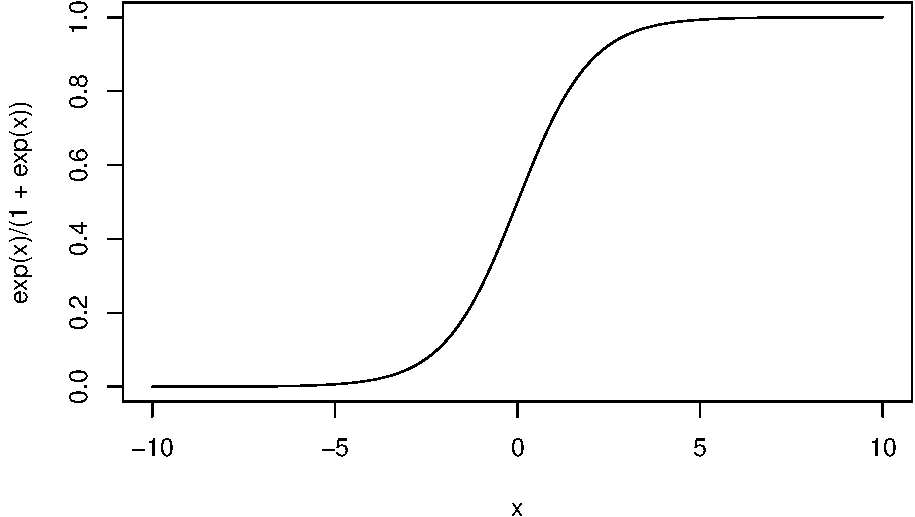
\includegraphics{Exercises_files/figure-latex/unnamed-chunk-1-1.pdf}

Essentially, what this means is that as there is no need for an insane
amount of pesticide because there is clearing a ceiling at which given
some x, the logistic link is approximately 1. The speed at which this
occurs is obviously different for different \(\vec{\beta}\). In this
case, \(\beta_1 = 0, \beta_2 = 1\).

\pagebreak

\subsection{Exercise Twelve}\label{exercise-twelve}

\paragraph{Questions and Solutions}\label{questions-and-solutions-1}

\emph{(Note: See Figure 3.3 for more relationships of distributions)}

\textbf{(a)}: Show that the Exponential distribution Exp\((\theta)\) is
a special case of the Gamma distribution G\((\alpha, \beta)\).

\emph{Solution: } The exponential distribution is
\(\text{Gamma}(1, 1/\theta)\).

\begin{align*}
G[\alpha, \beta] &= \frac{1}{\Gamma(\alpha)\beta^\alpha}x^{\alpha-1}e^{-x/\beta}\\
G[1, 1/\theta] &= \frac{1}{\Gamma(1)(1/\theta)^1}x^{1-1}e^{-x/(1/\theta)}\\
                &= \frac{1}{\theta^{-1}}x^0e^{-x\theta}\\
                &= \theta e^{-\theta x}\\
                &= \text{Exp}[\theta]
\end{align*}

\textbf{(b)}: If \(X\) has the Uniform Distribution U\([0,1]\) that is,
\(f(x) = 1\) for \(0 < x < 1\), show that \(Y = -\theta \log X\) has the
distribution Exp\((\theta)\).

\emph{Solution: }

\begin{align*}
\text{Exp}[\theta] &= \frac{1}{\theta} e^{- x/\theta}\\
X \sim \text{U}[0,1] &= 1\\
Y &= -\theta \log X\\
\implies X &= e^{-Y/\theta}\\
\frac{dX}{dY} &= \frac{-1}{\theta}e^{-Y/\theta}\\
f_Y(y) &= f_X(X)\left|\frac{dX}{dY}\right|\\
f_Y(y) &= \frac{1}{\theta}e^{-Y/\theta}\\
\end{align*}

\textbf{(c)}: Use the moment generating functions (or other methods) to
show

\begin{enumerate}
\def\labelenumi{\roman{enumi}.}
\tightlist
\item
  Bin\((n, \pi) \rightarrow \text{Po}(\lambda)\) as
  \(n \rightarrow \infty\)
\end{enumerate}

\emph{Solution: }

\begin{enumerate}
\def\labelenumi{\roman{enumi}.}
\setcounter{enumi}{1}
\tightlist
\item
  NBin\((r, \theta) \rightarrow \text{Po}(r(1 - \theta))\) as
  \(r \rightarrow \infty\)
\end{enumerate}

\emph{Solution: }

\textbf{(d)}: Use the Central Limit Theorem to show

\begin{enumerate}
\def\labelenumi{\roman{enumi}.}
\tightlist
\item
  \(\text{Po}(\lambda) \rightarrow \text{N}(\lambda, \lambda)\) for
  large \(\mu\).
\end{enumerate}

\emph{Solution: } \(\text{Po}(\lambda)\) can be thought of as the sum of
\(\lambda \text{ Po}(1)\) random variables. For large \(\mu\) then, the
distributed approaches the normal distribution with mean \(\mu\) and
standard deviation \(\sigma^2/n\) where \(\mu = \lambda\) and
\(\sigma^2 = \lambda^2\) and \(n\) being the sample size of \(\lambda\),
this reduces to \(\text{N}(\lambda, \lambda)\).

\begin{enumerate}
\def\labelenumi{\roman{enumi}.}
\tightlist
\item
  Bin\((n, \pi) \rightarrow\) N\((n\pi, n\pi(1 - \pi))\) for large
  \(n\), provided neither \(n\pi\) nor \(n\pi(1- \pi)\) is too small.
\end{enumerate}

The binomial distribution can be reduced to a sum of \(n\) Bernoulli
distributions distributed \(\text{Bernoulli}(p)\). The argument is
similar to \textbf{(a)}.

\begin{enumerate}
\def\labelenumi{\roman{enumi}.}
\tightlist
\item
  G\((\alpha, \beta) \rightarrow\) N\((\alpha/\beta, \alpha/\beta^2)\)
  for large \(\alpha\).
\end{enumerate}

The Gamma distribution can be reduced to the sum of \(\beta\)
Exponential distributions and follows a similar argument to
\textbf{(c)}.


\end{document}
